\documentclass{subfiles}
\begin{document}

    \paragraph{1. Main board}$~$\\
    First start with the main board of the bank. Cut two 20x18\SI{}{\square\centi\meter} pieces from W1.
    In the sapce left comes the walls arround your window.
    \begin{figure}[h]
        \centering
        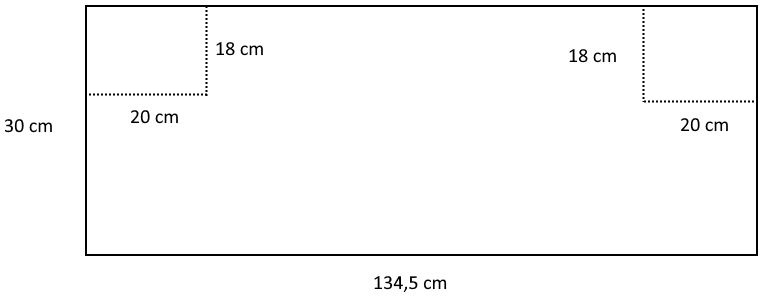
\includegraphics[width=0.5\textwidth]{Ressources/Cut_W1.png}
        \label{fig:Cut_W1}
        \caption{Cut out two 20x18\SI{}{\square\centi\meter} pieces from W1. }
    \end{figure}
    Keep the pieces, we can then reuse the wood to cut additional pieces. We define one as W1.1


    \paragraph{2. Triangle - Wall Protections}$~$\\
    We will now cut two long 20x4\SI{}{\square\centi\meter} wood on both side of W1.1. The goal is to 
    provide a protection between the wall and the metal triangles.
    \begin{figure}[h]
        \centering
        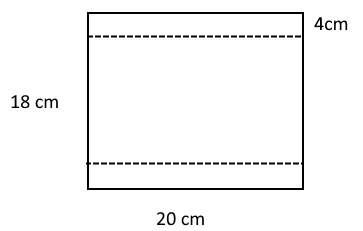
\includegraphics[width=0.5\textwidth]{Ressources/Cut_W1_1.png}
        \label{fig:Cut_W1_1}
        \caption{Cut two long 20x4\SI{}{\square\centi\meter} wood on both side of W1.1}
    \end{figure}
    You get two pieces that we define as W1.1.1 and W1.1.2.

    \paragraph{3. Rear Support}$~$\\
    We need support for the bank whene you on the rear of it to avoid falling back. 
    These piecies are fixed under the board and take support on the fixations of the railling to the walls. \newline
    
    We will now cut two small 10x5\SI{}{\square\centi\meter} wood in the rest of W1.1.
    \begin{figure}[h]
        \centering
        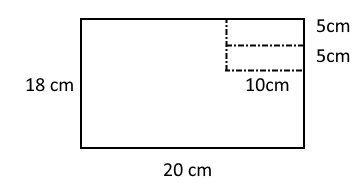
\includegraphics[width=0.5\textwidth]{Ressources/Cut_W1_1_3.png}
        \label{fig:Cut_W1_1_3}
        \caption{Cut two long 10x5\SI{}{\square\centi\meter} wood on both side of W1.1}
    \end{figure}
    You get two pieces that we define as W1.1.1 and W1.1.2.
\end{document}